%!TEX root = main.tex

\chapter{Background}
\label{chapter:background}

\section{Why hardware accelerators?}
\label{background:accel}


Recent trends in technology scaling, the availability of large amounts of data, and novel algorithmic breakthroughs have spurred accelerator architecture research.
In a general-purpose microprocessor, the overhead of instruction processing is much higher than the actual operations performed by each instruction.
This overhead includes the necessary steps to fetch and decode the instructions, provide required operands for the instructions, and perform the necessary bookkeeping to ensure correctness when multiple instructions are executing in the microprocessor.
Conversely, application specific hardware are faster and lower in power consumption than general-purpose processors because they eliminate most of the overhead of a general purpose processor~\cite{chung_micro_2010, hameed_asplos_2010_understanding}.
Although fixed-function accelerators are more energy efficient than software running a general-purpose processor, they are not a suitable solution for applications that change frequently.
As an alternative to fixed-function accelerators, reconfigurable architectures like field-programmable gate arrays (FPGAs) and coarse-grain reconfigurable architectures (CGRAs) have received renewed interest from academic researchers and industry practitioners alike, primarily due to their potential performance and energy efficiency benefits over conventional CPUs.
For instance, FPGAs are now being used to accelerate web search in datacenters at Microsoft and Baidu~\cite{catapult, baidu}, Amazon now offers FPGA instances as part of AWS~\cite{awsf1}, and Intel has announced products like in-package Xeon-FPGA systems~\cite{harp} and FPGA-accelerated storage systems~\cite{nand_flash}. Similarly, several recent research prototypes~\cite{dyser, triggered_instruction, scaledeep, scnn, plasticine, cgra_me} have explored various kinds of CGRAs at different granularity. Growing use of such reconfigurable architectures has made them more available to programmers now than ever before.
Although the flexibility of reconfigurable architectures enables changing the application by reconfiguring the accelerator, their programmability is still a major obstacle for their wide spread use.

\section{System-Design Challenges}


Reconfigurable devices, usually, accelerates part of the application which contains regular control flow and abundant data parallelism to achieve high performance and efficiency~\cite{spatial_computation, trips, govindaraju_hpca_2011}.
They can exploit: 1)multiple levels of nested parallelism, 2)data locality with custom data pipelines and 3)defining custom memory hierarchies.

Unfortunately, \textit{all the features that make reconfigurable architectures efficient also make them much more complex to program.}
For instance, in FPGAs, an accelerator design must account for the timing between pipelined signals and the physically limited compute and memory resources available on the target device.
It must also manage partitioning of data between local scratchpads and off-chip memory to achieve good data locality~\cite{gzip_2013_fpga}.


The combination of these complexities and market pressures, not the least
of which is reliability, we are finding that traditional design methods, in which
systems are designed directly at the low hardware or software levels, are fast
becoming infeasible~\cite{cascaval_taxonomy_accelerator}. This leads us to the well-known productivity gap generated by the disparity between the rapid paces at which design complexity has increased in comparison to that of design productivity~\cite{itrs}.
Figure~\ref{fig:productivity} shows the growth of design complexity and designer productivity
over time, as estimated by the Sematech in the mid-1990s. Design complexity
is fundamentally estimated by Moore’s Law, which predicts a 58%
annual increase in the number of transistors per chip. Sematech estimates that
designer productivity has grown and will continue to grow by only 21% per
year. The result is a wide and growing gap between the chips we can manufacture
and the chips we can design. 

\begin{figure}[h]
    \centering
    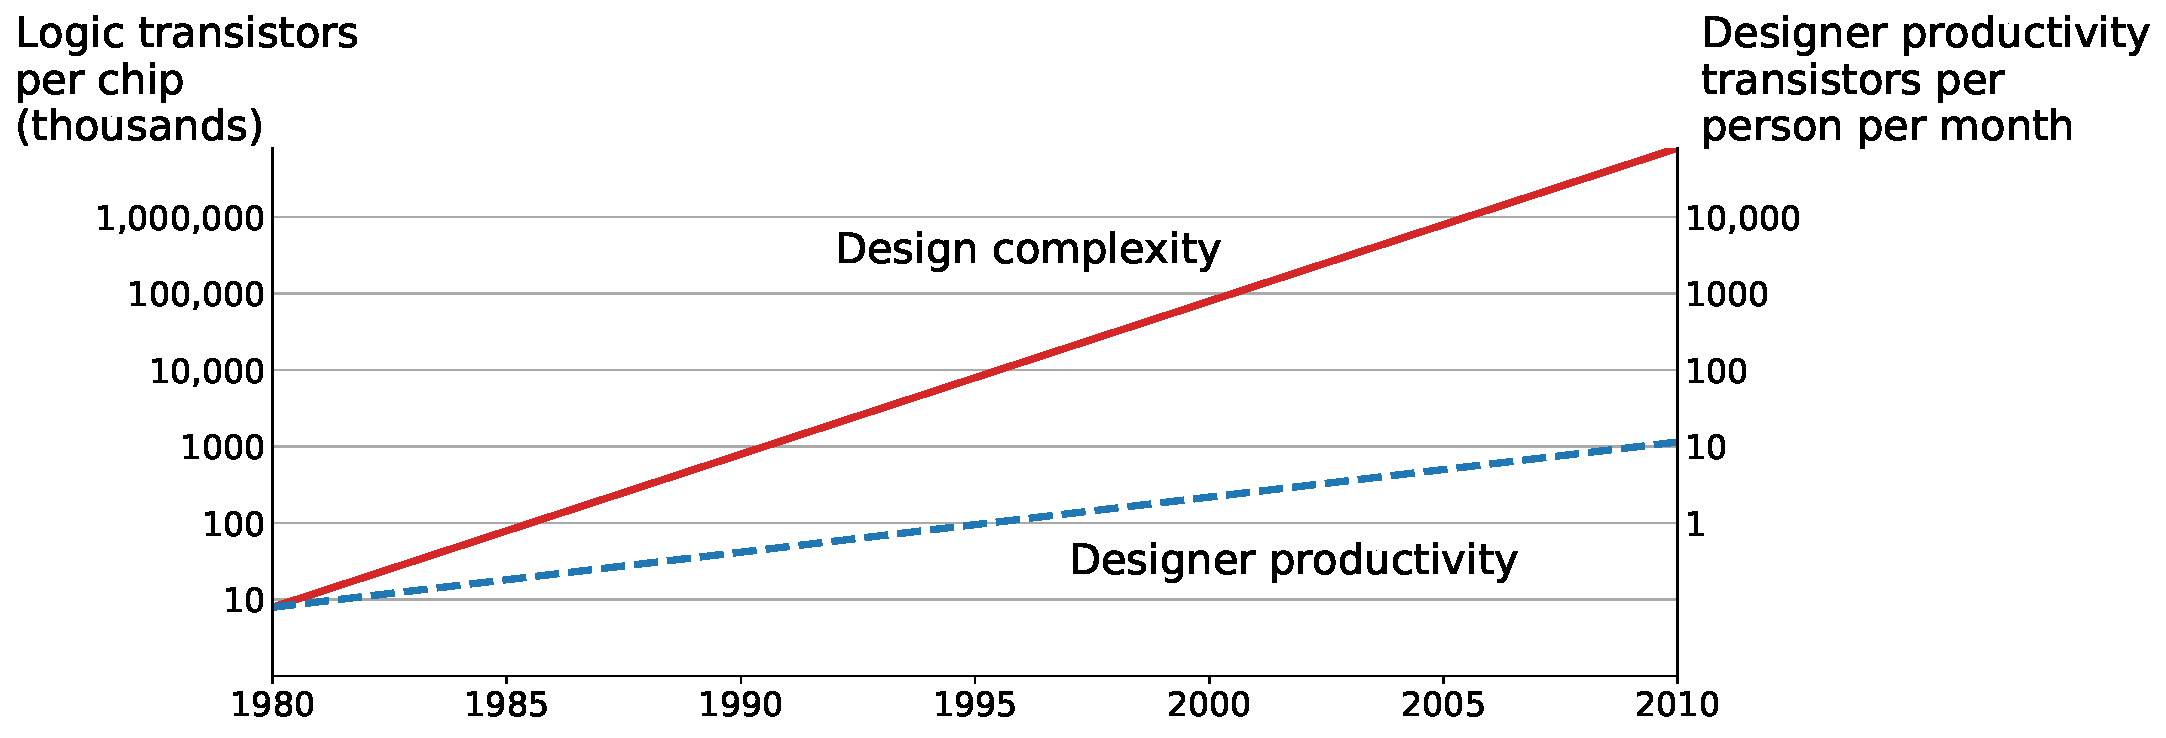
\includegraphics[width=\textwidth]{plots/productivity.pdf}
    \caption{Design complexity and designer productivity trends}
    \label{fig:productivity}
\end{figure}

One of the commonly-accepted solutions for closing the productivity gap as proposed by semiconductor roadmaps is to \emph{raise the level of abstraction in the design process.}
In order to achieve the acceptable productivity gains and to bridge the semantic gap between higher abstraction levels and low-level implementations, the goal now is to \emph{automate} the system-design process as much as possible.
However, to make automation possible we need to have: 1)A well-defined system abstraction level, well-known components of particular abstraction level and having a clear semantics for system-design languages.
The code, however, can be generated in a specific target language such as C>
In order to understand system-level possibilities more fully, we first explain the different abstraction levels involved in system design.
